\section{递归倾角滤波}
\label{sec:2.5}
递归滤波是一种将滤波输出反馈再作为输入的滤波形式。这种滤波只需微少计算时间即
可得出长的脉冲响应,在滑动平均的计算中特别有用。滑动平均可以实现频率域内的低通滤
波作用,但是一般最好还是避免进行空间变换。物理空间是比较方便的,它容许系数可变,
而且它允许更为灵活地处理边界问题。无论在空间域或时间域,地球物理数据组很少有在长
距离上呈平稳状态的,所以,递归滤波在统计估计问题中特别有用。

大多数滤波的目的都是想使被强同相轴所掩盖的重要的微弱同相轴有可能被观测到。一
维滤波仅靠对频率分量迸行选择或抑制才能作到这点;在二维情形下,则有可能采取一种不
同的准则,即倾角选择作用。

倾角滤波是地球物理学家长期以来感兴趣的一种处理(Embree, Burg及Backus,
1963)。陡倾角往往是地滚波干扰,水平倾角也可以是干扰。例如,弱断层绕射具有有价值
的信息,可是由于平缓地层的存在占主导优势,它们往往可能看不清楚。

要作普通的倾角滤波运算(扇形滤波),你只需将数据变换至($(\omega,k)$域,乘以任何
希望的与$k/\omega$有关之函数,然后再变换回去。扇形滤波就是这样对$k/\omega$倾角空间内的滤波响
应加以完全控制,而控制递归倾角滤波就不如此容易了,它们像扇形滤波一样可满足相同的
一般需要,而且还能提供下列的额外好处:
\begin{enumerate}
\item 时间可变性与空间可变性;
\item
  具有时间因果性;
\item
  易于实现;
\item
  计算时间比在$(\omega,k)$域内实现节省很多。
\end{enumerate}
时间因果性这种性质为进行数据记录提烘了一种有意义的可能,即可将水层速度截阻滤
波作用装进现代高密度海上电缆的记录装置内去进行,实现软件硬化。

\subsection{递归倾角滤波定义}
\label{sec:2.5.1}
令$P$表示原始数据,$Q$表示经过滤波处理之后的数据。当地震资料是准单频情形时,用
下列空间频率滤波可完成倾角滤波,其中,$\alpha$为可调截频参量:

%\begin{table}
%\centering
\begin{tabular}{|c|c|}
\hline
\multicolumn{2}{|c|}{单频资料情形下的倾角滤波($\omega\approx$常数)}\\ \hline
低通&$Q=\frac{a}{a+k^2}P$\\ \hline
高通&$Q=\frac{k^2}{a+k^2}P$ \\ \hline
\end{tabular}
%\end{table}

要在空间域内应用这些滤波,仅需将$k^2$解释为三对角线矩阵$\mathbf{T}$,其主对角线上的元素为
$(-1,2,-1)$。具体说,对于低通滤波,需要求解下述三对角线联立方程组
\begin{equation}
(\alpha\mathbf{I}+\mathbf{T})\mathbf{q}=\alpha\mathbf{p}
\label{eq:ex2.5.1}
\end{equation}
式中,$\mathbf{q}$与$\mathbf{p}$为列向量,其元素代表$x$轴上的不同位置(译注:式中的$\mathbf{I}$为单位矩阵)。以前求
解热流方程时,就已经用过这种矩阵。为使滤波是空间可变的,可取参量$\alpha$使与$x$有关,从而可
用一种任意的对角线矩阵来代替$\alpha\mathbf{I}$。究竟是在频率$\omega$域内还是在时间$t$域内来表示$\mathbf{p}$与$\mathbf{q}$,没什
么关系。

现在从狭频带资料转而注意具有较宽一点的'频谱之资料,这时可参考下述滤波:

%\begin{table}
%\centering
\begin{tabular}{|c|c|}
\hline
\multicolumn{2}{|c|}{中等频带宽度($\Delta\omega$)资料情形下的倾角滤波} \\ \hline
低通&$Q=\frac{a}{a+\frac{k^2}{-i\omega}}P$\\ \hline
高通&$Q=\frac{\frac{k^2}{-i\omega}}{a+\frac{k^2}{-i\omega}}P$ \\ \hline
\end{tabular}\\
%\caption{2.5.2}
%\label{tab:2.5.2}
%\end{table}
为了解这些滤波作用,注意下$(\omega,k)$平面内$k^2/\omega$为常数时,即$\omega\approx k^2$时的等值
线。如图\ref{fig:txz/dipfil}所示之例子,这样一些等值线
都属于具有恒定阻尼和恒定相移的曲线。低通
滤波\footnote{所谓“低通”,是指低视倾角可通过而高视倾角被截止。——译者}通带内没有相移,不过在阻尼带内有时
间微分。根据前面给出的定义方程,这个结论
是很显然的。高通滤波在平缓的通带内没有相移,但是在阻尼带内有时间积分。
\begin{figure}[H]
\centering
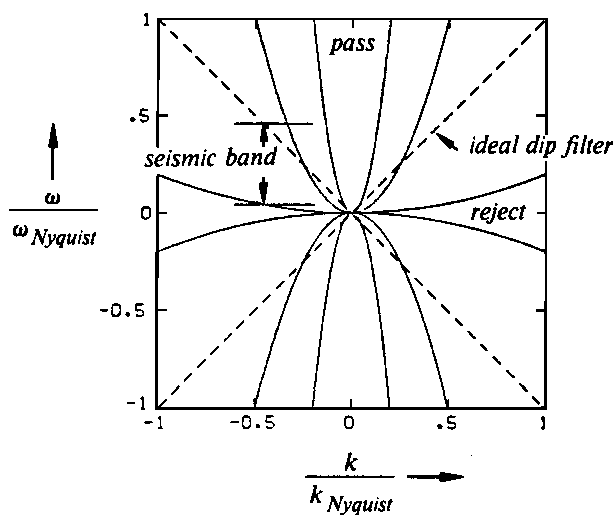
\includegraphics[width=0.65\textwidth]{txz/dipfil}
\caption[dipfil]{倾角滤波的恒定阻尼等值线在地震频带范围内,这些抛物线均可满意地近似与图中的
虚线直线(理想倾角滤波)。图中,通带与阻带均指低通滤波情形(Hale)}
\label{fig:txz/dipfil}
\end{figure}
这些倾角滤波的一个有趣的特点就是,低
通与高通滤波构成一对其稆等于1的滤波。所
以,如果一个数据组被它们分别滤波然后相
加,原封不动什么也不会损失。反之,一旦计
算出低通滤波后的输出,就能非常容易地计算
出高通滤波输出,因为只要从输入中减去低通输出就行了。

\subsection{递归倾角滤波的实现}
\label{sec:2.5.2}
实现中等频宽倾角滤波也是很方便的事。

例如,消去分母,低通滤波就变成下式:
\begin{equation}
(-i\omega\alpha\mathbf{I}+\mathbf{T})\mathbf{Q}=-i\omega\alpha\mathbf{P}
\label{eq:ex2.5.2}
\end{equation}
主要诀窍在于:在Crank-Nicolson意义下实现与$-i\omega$如所对应的微分过程。那就是说,未经
微分的诸项要按相邻的值加以平均,即
\begin{equation}
\mathbf{I}\frac{\alpha}{\Delta t}(\mathbf{q}_{t+1}-\mathbf{q}_{t})+
\mathbf{T}\frac{\mathbf{q}_{t+1}+\mathbf{q}_{t}}{2}=
\frac{\alpha}{\Delta t}(\mathbf{p}_{t+1}+\mathbf{p}_{t})
\label{eq:ex2.5.3}
\end{equation}
将未知数集中于左端,得
\begin{equation}
\mathbf{I}\frac{\alpha}{\Delta t}\mathbf{q}_{t+1}=
(\frac{\alpha}{\Delta t}\mathbf{I}-\frac{1}{2}\mathbf{T})\mathbf{q}_{t}+
\frac{\alpha}{\Delta t}(\mathbf{p}_{t+1}+\mathbf{p}_{t})
\label{eq:ex2.5.4}
\end{equation}
式\ref{eq:ex2.5.4}是一个关于未知数$\mathbf{q}_{t+1}$的三对角线联立方程组,能对相继的$t$值递归解出该方程组。

参量$\alpha$决定截频,它可取为时间与空间的任何函数。不过,如果该函数变化极迅速,这
时可能有必要结合某种稳定性分析,综合加以考虑。由于要利用波动方程,这种稳定性分析
将在以第\ref{chap:offset}章中讨论。

\subsection{侧边界影响}
\label{sec:2.5.3}

地球物理学家通常希望最好不存在侧边界,或者它们无限远离。有两类侧边界条件要加
以考虑,一是沿$x$方向的边界,一是沿$k$方向的边界条件。

用零斜率侧边界条件总能最好地近似在x方向上的侧边条件。由于我们以前已经学习过
求解任何三对角线方程组,所以有可能利用更为一般性的侧边界条件。

$k$空间内的侧边界条件与最陡的倾角有关,处理这些倾角的一种途径是利用$\mathbf{T}/
(l-\beta\mathbf{T})$
来代替$k^2$,这要引进另一个可调参量$\beta$它必须保持小于1/4,细节将在\ref{sec:4.3}节内讨论。

\subsection{扇形滤波}
\label{sec:2.5.4}

我们当然愿意用真正的倾角滤波,即采用$k/\omega$的函数而不是采用上述的函数,但
是,可以证明,在上述各表达式中用$k^2/\omega^2$代替$k^2/\omega$,它们的递归计算过程都是不稳定
的。

通过Hale与Claerbout(1983)曾阐述过的种种近似方法可以定义锐截止扇形滤波(更
严格讲,这些滤波都是$k/\omega$的某种矩形函数)。一般而言,可将$\mid k\mid$展开成$\partial^2/\partial x^2$的幂级数,
如果对$\mid k\mid$的近似保证是正的,你就有望便代表$\mid k\mid i\omega$的递归具有稳定性。

更简单的情形是,你也许乐意对时间域或者空间域作傅氏变换,而不是二者都作,在末
作变换的那一个域内。要求作高通或低通滤波运算,这时采用诸如Butterworth滤波等种种
技术很容易就能作到。

\subsection{高维情形}
\label{sec:2.5.5}

很自然会想到,递归的三维低通倾角滤波可用下述函数形式:
\begin{equation}
\frac{\alpha}{\alpha+\frac{k_x^2+k_y^2}{-i\omega}}
\label{eq:ex2.5.5}
\end{equation}
然而,这种滤波采甩Crank-Nicolson算法是办不到的事。利用下式:
\begin{equation}
(\frac{\alpha_x}{\alpha_x+\frac{k_x^2}{-i\omega}})(\frac{\alpha_y}{\alpha_y+\frac{k_y^2}{-i\omega}})
\label{eq:ex2.5.6}
\end{equation}
